

\section{Statistics of LLM-Generated Specifications}
\label{appendix:sat}


\begin{figure}[h]
  \centering
  \begin{subfigure}[b]{0.49\linewidth}
    \centering
    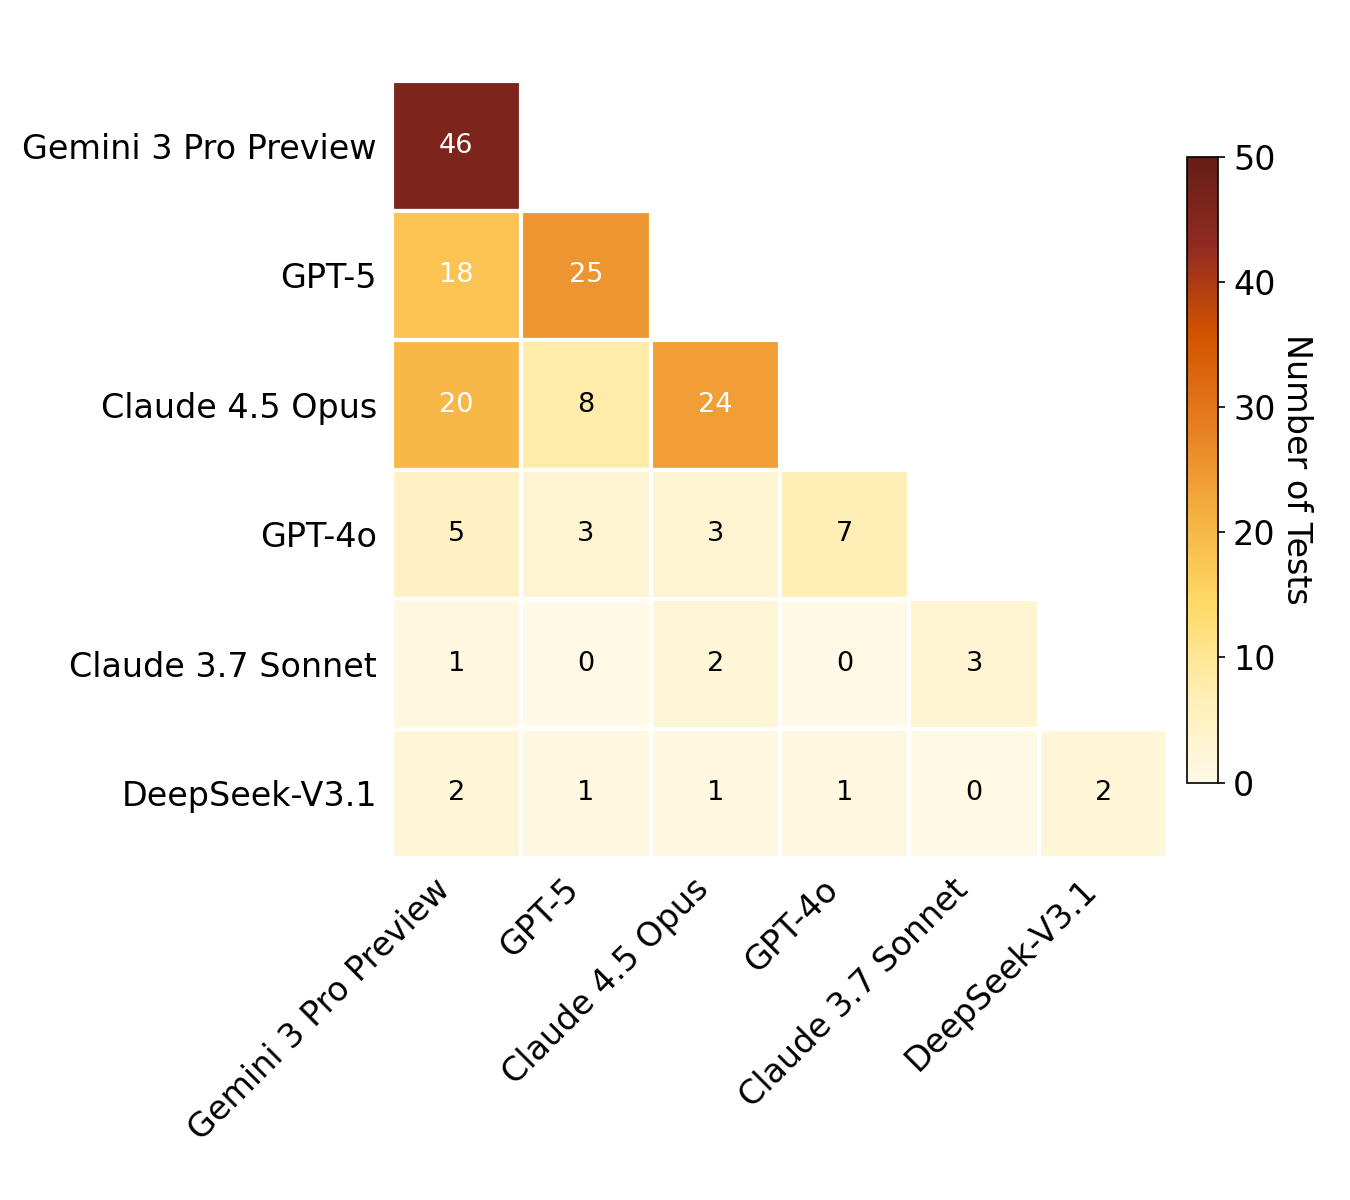
\includegraphics[width=\linewidth]{images/heatmap.png}
    \caption{Pairwise intersection of candidates.}
    \label{fig:intersection}
  \end{subfigure}
  \hfill
  \begin{subfigure}[b]{0.49\linewidth}
    \centering
    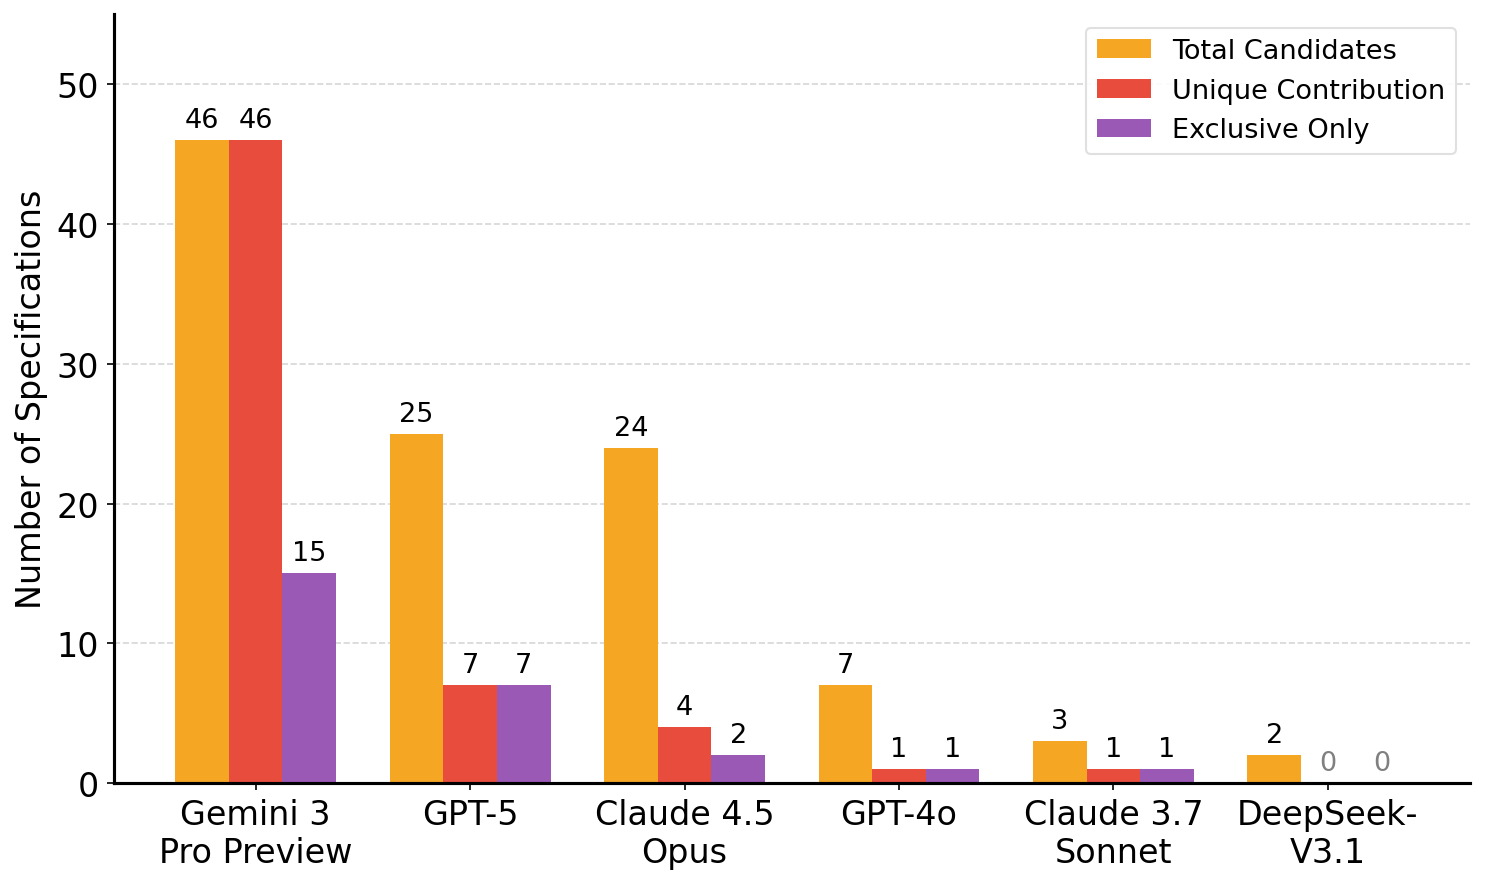
\includegraphics[width=\linewidth]{images/unique.png}
    \caption{Statistics of generated specifications per model.}
    \label{fig:unique}
  \end{subfigure}
  \caption{Model performance on candidate specification generation. (a) Diagonal entries show each model's total candidates; off-diagonal entries show shared successes. (b) Total candidates, unique contributions to the aggregated set, and exclusive successes (solved by that model only).}
  \label{fig:model_comparison}
\end{figure}


Figure~\ref{fig:model_comparison} reports detailed statistics of candidate specifications generated by each LLM. We analyze both the total number of valid specifications per model and their overlap structure to better understand model complementarity under our aggregation strategy.

Figure~\ref{fig:intersection} presents the pairwise intersection matrix. Diagonal entries correspond to the total number of valid specifications produced by each model, while off-diagonal entries indicate shared successes. The results reveal substantial but incomplete overlap among top-performing models. Gemini~3~Pro~Preview shares 18 specifications with GPT-5 and 20 with Claude~4.5~Opus, reflecting its broad coverage. In contrast, GPT-5 and Claude~4.5~Opus share only 8 specifications despite having comparable total counts, indicating that they capture different regions of the specification space. Lower-performing models exhibit limited overlap both with each other and with the top-tier models, and their successes are largely subsumed by stronger models.

Figure~\ref{fig:unique} further decomposes each model’s contribution into total candidates, unique contributions to the aggregated set, and exclusive successes (i.e., problems solved only by that model). Gemini~3~Pro~Preview achieves the strongest performance with 46 valid specifications, including 15 exclusive successes not covered by any other model. GPT-5 and Claude~4.5~Opus generate 25 and 24 valid specifications, respectively; however, GPT-5 contributes more exclusive specifications (7 vs.\ 2), suggesting greater diversity relative to other models. The remaining models—GPT-4o, Claude~3.7~Sonnet, and DeepSeek-V3.1—produce only a small number of valid specifications and add limited unique coverage.

Overall, these statistics motivate our priority-based aggregation strategy described in the main text. Although individual models differ in overall capability, their partial overlap and complementary strengths imply that no single model dominates across all problems. Aggregating candidates by model ranking therefore improves overall coverage while retaining the highest-quality specification available for each problem.
